%	First attempt at making PhD Thesis template in LaTeX.
%	Western Sydney University PhD Thesis Template
%	Copyright (C) 2017-2018  Samuel J. Frost
%	Email: samuel.frost.1991@gmail.com
%
%	This program is free software: you can redistribute it and/or modify
%	it under the terms of the GNU General Public License as published by
%	the Free Software Foundation, either version 3 of the License, or
%	(at your option) any later version.
%
%	This program is distributed in the hope that it will be useful,
%	but WITHOUT ANY WARRANTY; without even the implied warranty of
%	MERCHANTABILITY or FITNESS FOR A PARTICULAR PURPOSE.  See the
%	GNU General Public License for more details.
%
%	You should have received a copy of the GNU General Public License
%	along with this program.  If not, see <http://www.gnu.org/licenses/>.
%
%	========================================================================
%	
%	The initial set-up of the document class. Experimenting with book format
%	to begin with. Change 'twoside' to 'oneside' to go from having print
%	on both sides to only on the right. The 'openright' command forces title
%	pages to only be on the right hand side. 

	\documentclass[12pt,openright,twoside]{report} % remove twoside to make like book
	\renewcommand{\baselinestretch}{2}	% 1.5 spacing
	\usepackage{fancyhdr}
		\fancyheadoffset{0pt}
		\fancyhead{}
		\fancyhead[RO]{A Western Sydney University Thesis Template} % add ,LE for same on both pages
		\fancyfoot{}
		\fancyfoot[LE,RO]{\thepage}
		\fancyfoot[LO,RE]{Chapter \thechapter}
		\fancyfoot[CO,CE]{Your Name}
		\renewcommand{\headrulewidth}{0.4pt}
	   	\renewcommand{\footrulewidth}{0.4pt}
	\usepackage{graphicx}					% graphics management
		\graphicspath{ {Figures/} }			% folder where figures are stored in parent directory
	\usepackage{layout}
	\usepackage{indentfirst}				% indentation at start of paragraph
	\usepackage[a4paper,width=150mm,top=25mm,bottom=25mm,bindingoffset=15mm,textwidth=450pt,textheight=650pt]{geometry}						% paper set-up	
	\usepackage{lscape}
	\usepackage[osf,sc]{mathpazo}			% to stop equations being italicised
	\usepackage{eulervm}					
	\usepackage[labelfont=bf]{caption}		% bold figure number title	
	\usepackage{float}
	\usepackage{booktabs}
	\usepackage{multirow}
	\usepackage{cite}						% main reason is to join references together i.e. [1-3] instead of [1,2,3]
	\bibliographystyle{unsrt}			 % unsrt also okay
	\renewcommand{\bibname}{References}		% change name of bibliography to references
	\usepackage[nottoc]{tocbibind}			% to include references in bibliography remove numbib to remove chapter number
	\usepackage{pdfpages}
	\usepackage{enumitem}					% bold numbers in numerical list
	\usepackage{ragged2e}					% for justifying text after \centering
	\usepackage{lipsum}							% only for filling template with text
%
%	
%	========================================================================

\title{A Western Sydney University Thesis Template}	% running title - insert your title here
\author{Your Name} %replace with your name
\date{2018}
\begin{document}
	\pagenumbering{roman} % switch between roman and arabic when desired
	\cleardoublepage
\renewcommand{\baselinestretch}{1.5}
\begin{titlepage}
    \begin{center}
        \vspace*{1cm}
        
\includegraphics[width=1\textwidth]{wsu-logo-large.png}
         \LARGE
        \textbf{A WESTERN SYDNEY UNIVERSITY THESIS TEMPLATE} %your title here
        \vspace{1cm}
        
        \large\textbf{Your Name}
        
        \vspace{0.25cm}
        \normalsize
        In fulfilment of the requirements\\
        for the degree of Doctor of Philosophy
        
        \vspace{0.25cm}
        
 
        
\includegraphics[width=0.4\textwidth]{WSU_logo.png}
        \vfill
    
              
        \large
        School of Science and Health\\
        Western Sydney University\\
        Australia\\
        March 2018
        
    \end{center}
\end{titlepage}
 % ensure your folder structure and file names are called correctly
	\renewcommand{\baselinestretch}{2} % switching between different text-spacing - there are more efficient ways of doing so
	\cleardoublepage
	\chapter*{Acknowledgements}
\addcontentsline{toc}{chapter}{Acknowledgements}
\thispagestyle{plain}

\lipsum[1-2]
	\chapter*{Statement of Authenticity}
 \addcontentsline{toc}{chapter}{Statement of Authenticity}
 \thispagestyle{plain}


This thesis is submitted in fulfilment of the requirements for Doctorate of Philosophy (Science) at Western Sydney University. The work presented in this thesis is, to the best of my knowledge and belief, original except as acknowledged in the text. I hereby declare that I have not submitted this material, either in full or in part, for a degree at this or any other institution. 
 
 \vspace{1cm}
 \begin{flushright}
 	\hspace{10cm}\hrulefill\\
 	\vspace{0.5cm}
 	\large
 	\textbf{Your Name}
 \end{flushright}
 							% statement of authenticity
	\clearpage
	\chapter*{Publications}
 \addcontentsline{toc}{chapter}{Publications}
  \thispagestyle{plain}


\vspace*{\fill}
\begin{enumerate}[label=\textbf{(\roman*)}]
	
	\item \textbf{Name, Y.} Publication 1
	\item \textbf{Name, Y.} Publication 2
	\item \textbf{Name, Y.} Publication 3
	
\end{enumerate}
\vspace*{\fill}
	\renewcommand{\baselinestretch}{1.5}\normalsize
	\tableofcontents
	\listoffigures
	\listoftables
	\chapter*{Abbreviations}
 \addcontentsline{toc}{chapter}{Abbreviations}
  \thispagestyle{plain}
  % I kept the abbreviations as a table in this instance, feel free to use any method you like
\begin{table}[!ht]
	\resizebox{.95\textwidth}{!}{%
\begin{tabular}{llll}
	\textbf{\boldmath{$\lambda$}}     & Wavelength (nm)                & \textbf{NRs}                           & Nanorods                             \\
	\textbf{\textbf{\boldmath$\mu$L}} & Microliters                    & \textbf{OFM}                           & Ovine Forestomach Matrix             \\
	\textbf{\textbf{\boldmath$\mu$m}} & Micrometers                    & \textbf{Pa}                            & Pascals                              \\
	\textbf{\textbf{\boldmath$\mu$N}} & Micronewtons                   & \textbf{PDMS}                          & Polydimethylsiloxane                 \\
	\textbf{$^\circ$C}                & Degrees Celsius                & \textbf{PDT}                           & Photodynamic Therapy                 \\
	\textbf{AFM}                      & Atomic Force Microscopy        & \textbf{PGSA}                          & Poly(glycerol sebacate acrylate)     \\
	\textbf{bFGF}                     & Basic Fibroblast Growth Factor & \textbf{PMMA}                          & Poly(methyl methacrylate)            \\
	\textbf{BSE}                      & Back-Scattered Electron        & \textbf{PS}                            & Photo-Sensitiser                     \\
	\textbf{cm}                       & Centimeters                    & \textbf{PS-b-PAA}                      & polystyrene-block-poly(acrylic acid) \\
	\textbf{ECM}                      & Extracellular Matrix           & \textbf{PTB}                           & Photochemical Tissue Bonding         \\
	\textbf{FG}                       & Fibrin Glue                    & \textbf{RB}                            & Rose Bengal                          \\
	\textbf{FGF}                      & Fibroblast Growth Factor       & \textbf{ROS}                           & Reactive Oxygen Species              \\
	\textbf{ICG}                      & Indocyanine Green              & \textbf{s}                             & Seconds                              \\
	\textbf{IR}                       & Infrared                       & \textbf{SD}                            & Standard Deviation                   \\
	\textbf{J}                        & Energy (Joules)                & \textbf{SEM}                           & Scanning Electron Microscopy         \\
	\textbf{kPa}                      & Kilopascals                    & \textbf{SIS}                           & Small Intestinal Submucosa           \\
	\textbf{LED}                      & Light Emitting Diode           & \textbf{T}                             & Temperature                          \\
	\textbf{LTR}                      & Laser Tissue Repair            & \textbf{TEM}                           & Transmission Electron Microscopy     \\
	\textbf{LTW}                      & Laser Tissue Welding           & \textbf{\textbf{TGF-\boldmath$\beta$}} & Transforming Growth Factor $\beta$   \\
	\textbf{MMW}                      & Medium Molecular Weight        & \textbf{UV}                            & Ultraviolet                          \\
	\textbf{mN}                       & Millinewtons                   & \textbf{v/v}                           & Volume to Volume                     \\
	\textbf{MPa}                      & Megapascals                    & \textbf{vdW}                           & van der Waals                        \\
	\textbf{mW}                       & Power (Milliwatts)             & \textbf{VEGF}                          & Vascular Endothelial Growth Factor   \\
	\textbf{N}                        & Newtons                        & \textbf{W}                             & Power (Watts)                        \\
	\textbf{nm}                       & Nanometers                     & \textbf{w/v}                           & Weight to Volume                     \\
	\textbf{NMR}                      & Nuclear Magnetic Resonance     & \textbf{wt \%}                         & Weight Solute/Weight Solvent         \\
	\textbf{NPs}                      & Nanoparticles                  & \textbf{}                              &                                     
\end{tabular}
}
\end{table}
	\renewcommand{\baselinestretch}{2}\normalsize
	\cleardoublepage
	 \chapter*{Abstract}
 \addcontentsline{toc}{chapter}{Abstract}
 \thispagestyle{plain}

\lipsum[1-5]

	\chapter{The First Chapter} \label{Chapter 1}
	\pagestyle{fancy}
	\pagenumbering{arabic}
		\begin{figure}[!h]
		\centering
		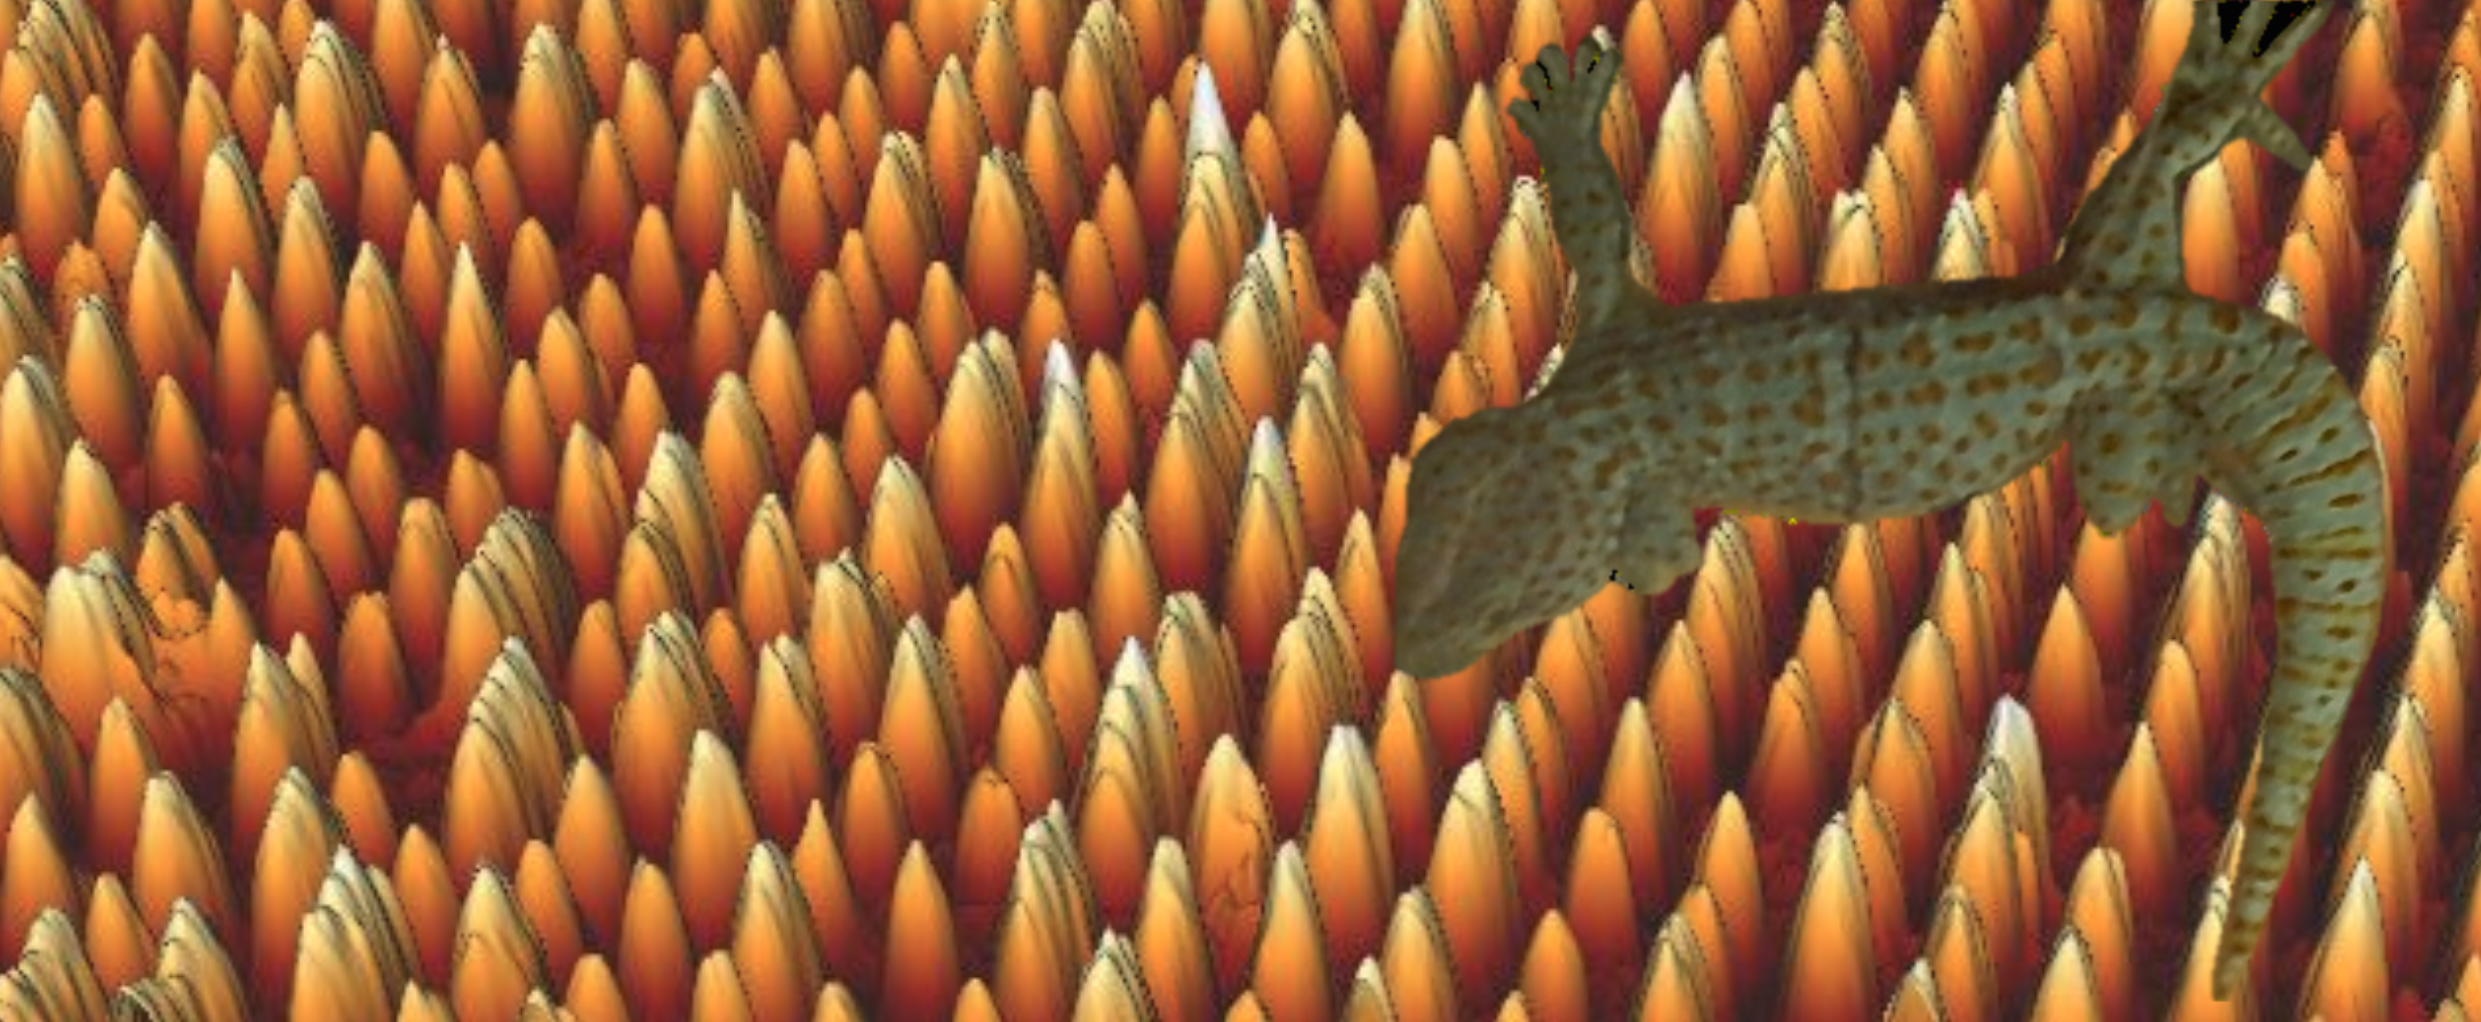
\includegraphics[width=\textwidth]{chapter1abs}	
		\end{figure}
	\noindent The way this page is presented shows how I structured my chapters. Each chapter had a graphical abstract (above) and was a based on a publication. The text here was replaced with the citation, and description of what I had contributed to the manuscript. Feel free to use your own design here.
	\clearpage
	 \section{Introduction}
 
\lipsum[5-7] Image shows an image.

 \renewcommand{\baselinestretch}{1.5}
\begin{figure}[!htbp]
	\centering
	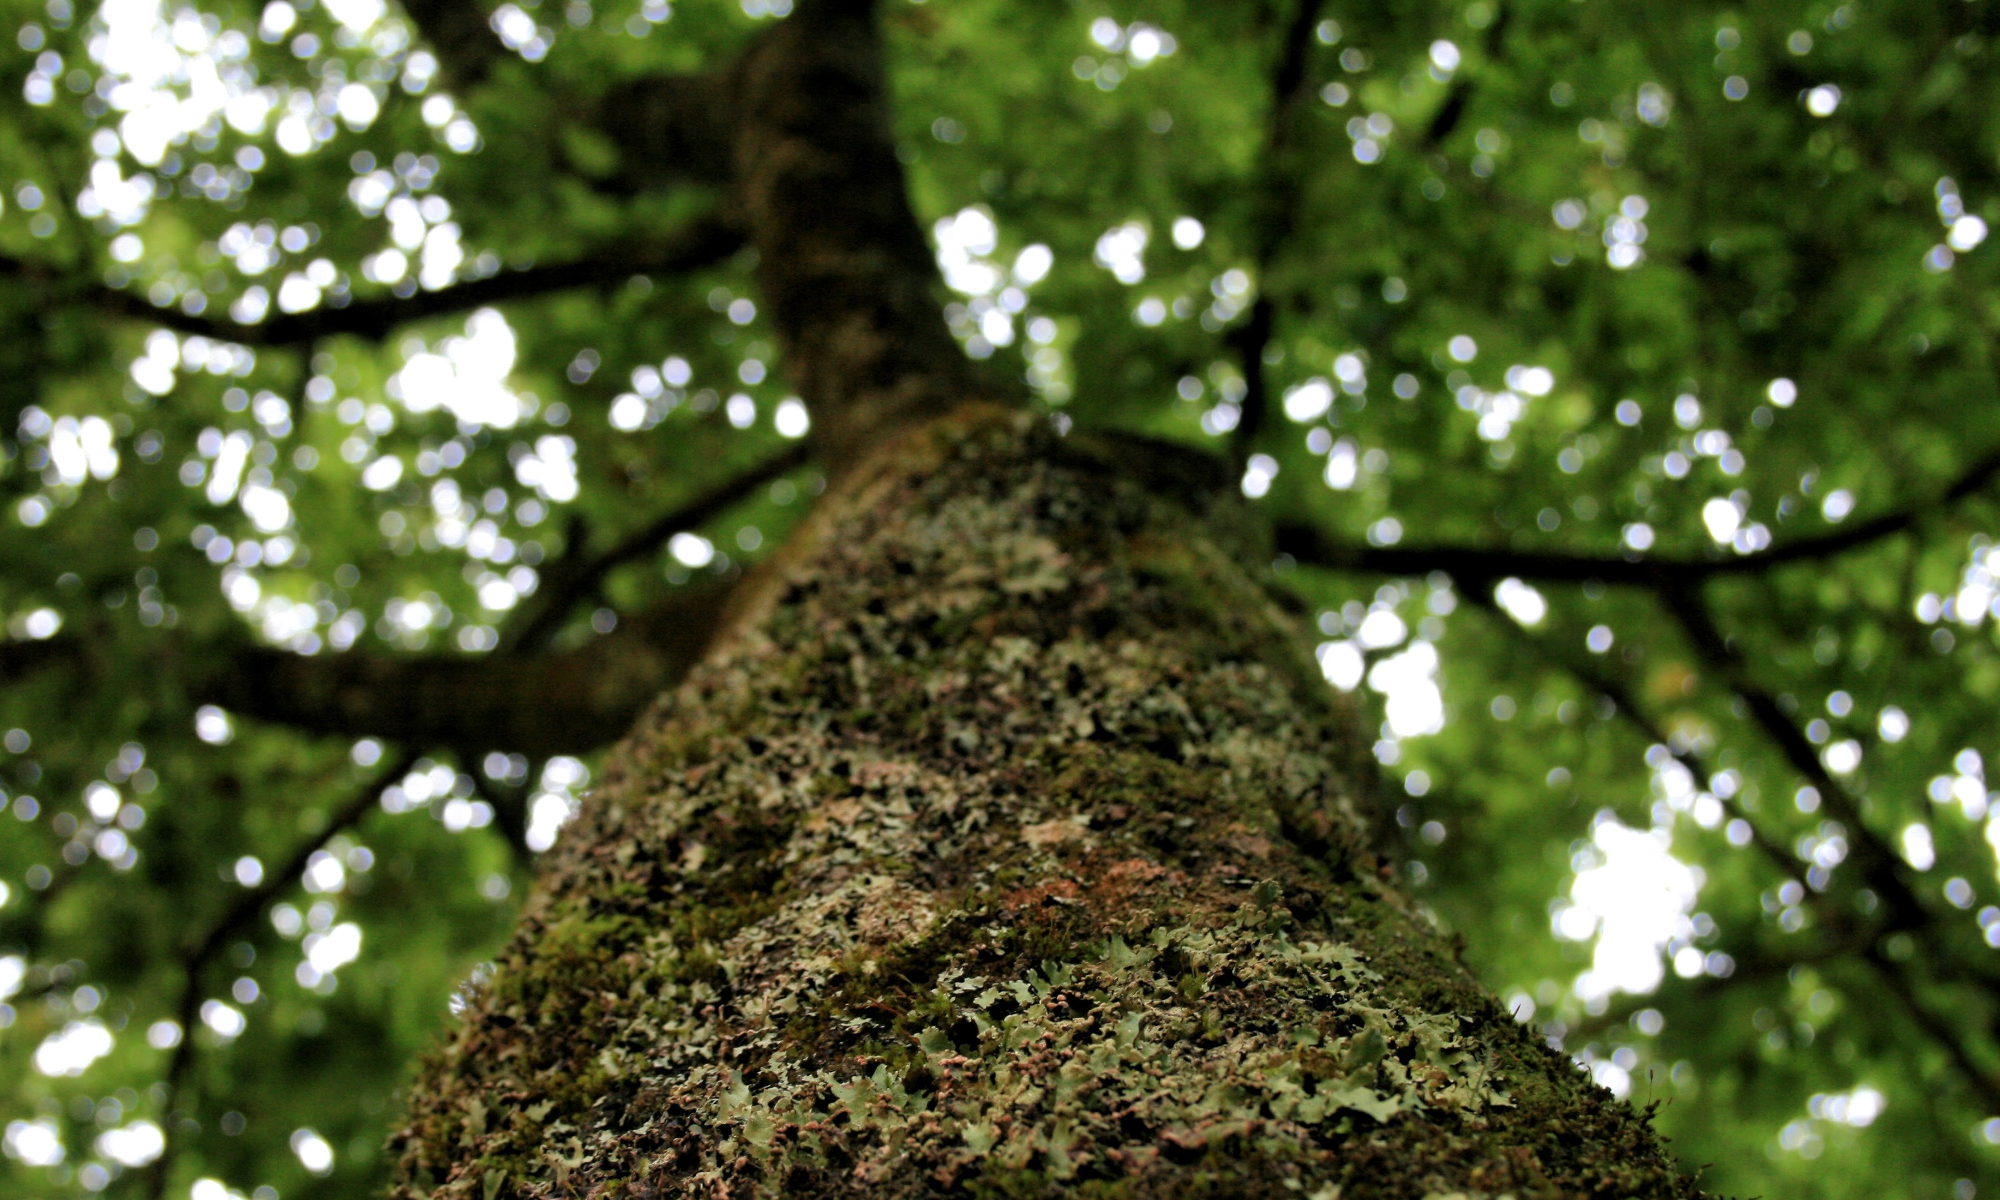
\includegraphics[width=\textwidth]{chapter1figure1}
	\caption[This title will appear in the TOC]{This is a longer more descriptive image caption.}
	\label{fig:chapter1figure1}		
\end{figure}
\renewcommand{\baselinestretch}{2.0}

\lipsum[7-8]
 
 
\section{Next Section}
 
\lipsum[9-10] Equation \ref{eqn:force} shows the fundamental relationship between force, mass, and acceleration. 

 	\begin{equation}
	F = m\times a
	\label{eqn:force}
	\end{equation}
	
\lipsum[11]

\subsection{Sub-Section}

\lipsum[1]. Table \ref{chapter1table1} is an example of a horizontal table on a landscape page.

\renewcommand{\baselinestretch}{1.5}
\begin{landscape}
	\begin{table}[p]
 		\centering
		\caption{This Is A Table}
		\label{chapter1table1}
		\resizebox{.8\textwidth}{!}{% based on the table you can change the multiplier for text width to fill as much or as little of the page as you want
\begin{tabular}{@{}ccccc@{}}
	\toprule
	\textbf{Section 1} & \textbf{Section 2} & \textbf{Section 3} & \textbf{Section 4} & \textbf{Section 5} \\ \midrule
	\textbf{1}         & Red                & Blue               & Green              & Yellow             \\
	\textbf{2}         & Orange             & Red                & Blue               & Green              \\
	\textbf{3}         & Yellow             & Orange             & Red                & Blue               \\
	\textbf{4}         & Green              & Yellow             & Orange             & Red                \\
	\textbf{5}         & Blue               & Green              & Yellow             & Orange             \\
	\textbf{6}         & Red                & Blue               & Green              & Yellow             \\
	\textbf{7}         & Orange             & Red                & Blue               & Green              \\
	\textbf{8}         & Yellow             & Orange             & Red                & Blue               \\
	\textbf{9}         & Green              & Yellow             & Orange             & Red                \\ \bottomrule
\end{tabular}%
}
	\begin{center}
	\small This is the caption of the table.
	\end{center}
\end{table}
\end{landscape}
\renewcommand{\baselinestretch}{2}
 
The following is a list:
\begin{enumerate}[label=\textbf{(\arabic*)}]
 	\item This
 		\item Is
 			\item A
 				\item List
  \end{enumerate}
 
 
 
 
 

	\chapter{The Next Chapter} \label{Chapter 2}
	% feel free to change the style of your chapter openings, but, remember to keep it consistent
	\section{Abstract}
\lipsum[1]
\section{How To Reference}
For you referencing I used Zotero to keep track of all of my citations. From Zotero you can then export your library as BibTeX into the parent directory of your thesis (in my case as references.bib). This is an example of a single citation \cite{frost_gecko-inspired_2016}. This is an example of multiple citations \cite{frost_gecko-inspired_2016,frost_micro_2016,frost_semitransparent_2018}. You can change the referencing style in the preamble in \textit{thesis-main.tex}.
	
	
	\chapter{Conclusions}
	\lipsum[1-4]

	\renewcommand{\baselinestretch}{1.5}\normalsize
	\bibliography{references}
	\renewcommand{\baselinestretch}{2}\normalsize
	\clearpage
	
	\appendix
	
	\chapter{Appendix 1}
	This is where your supporting information would go. Include tables, data, etc.
	
	\chapter{Paper 1} \label{Appendix 2}
	\noindent {\Large Include Any Published Papers Easily In Your Appendices}
	\newline
	\noindent Be sure to request permissions from journal and include that permission here. I have just imported the source code for thesis-main.tex as a pdf to demonstrate. 
	
	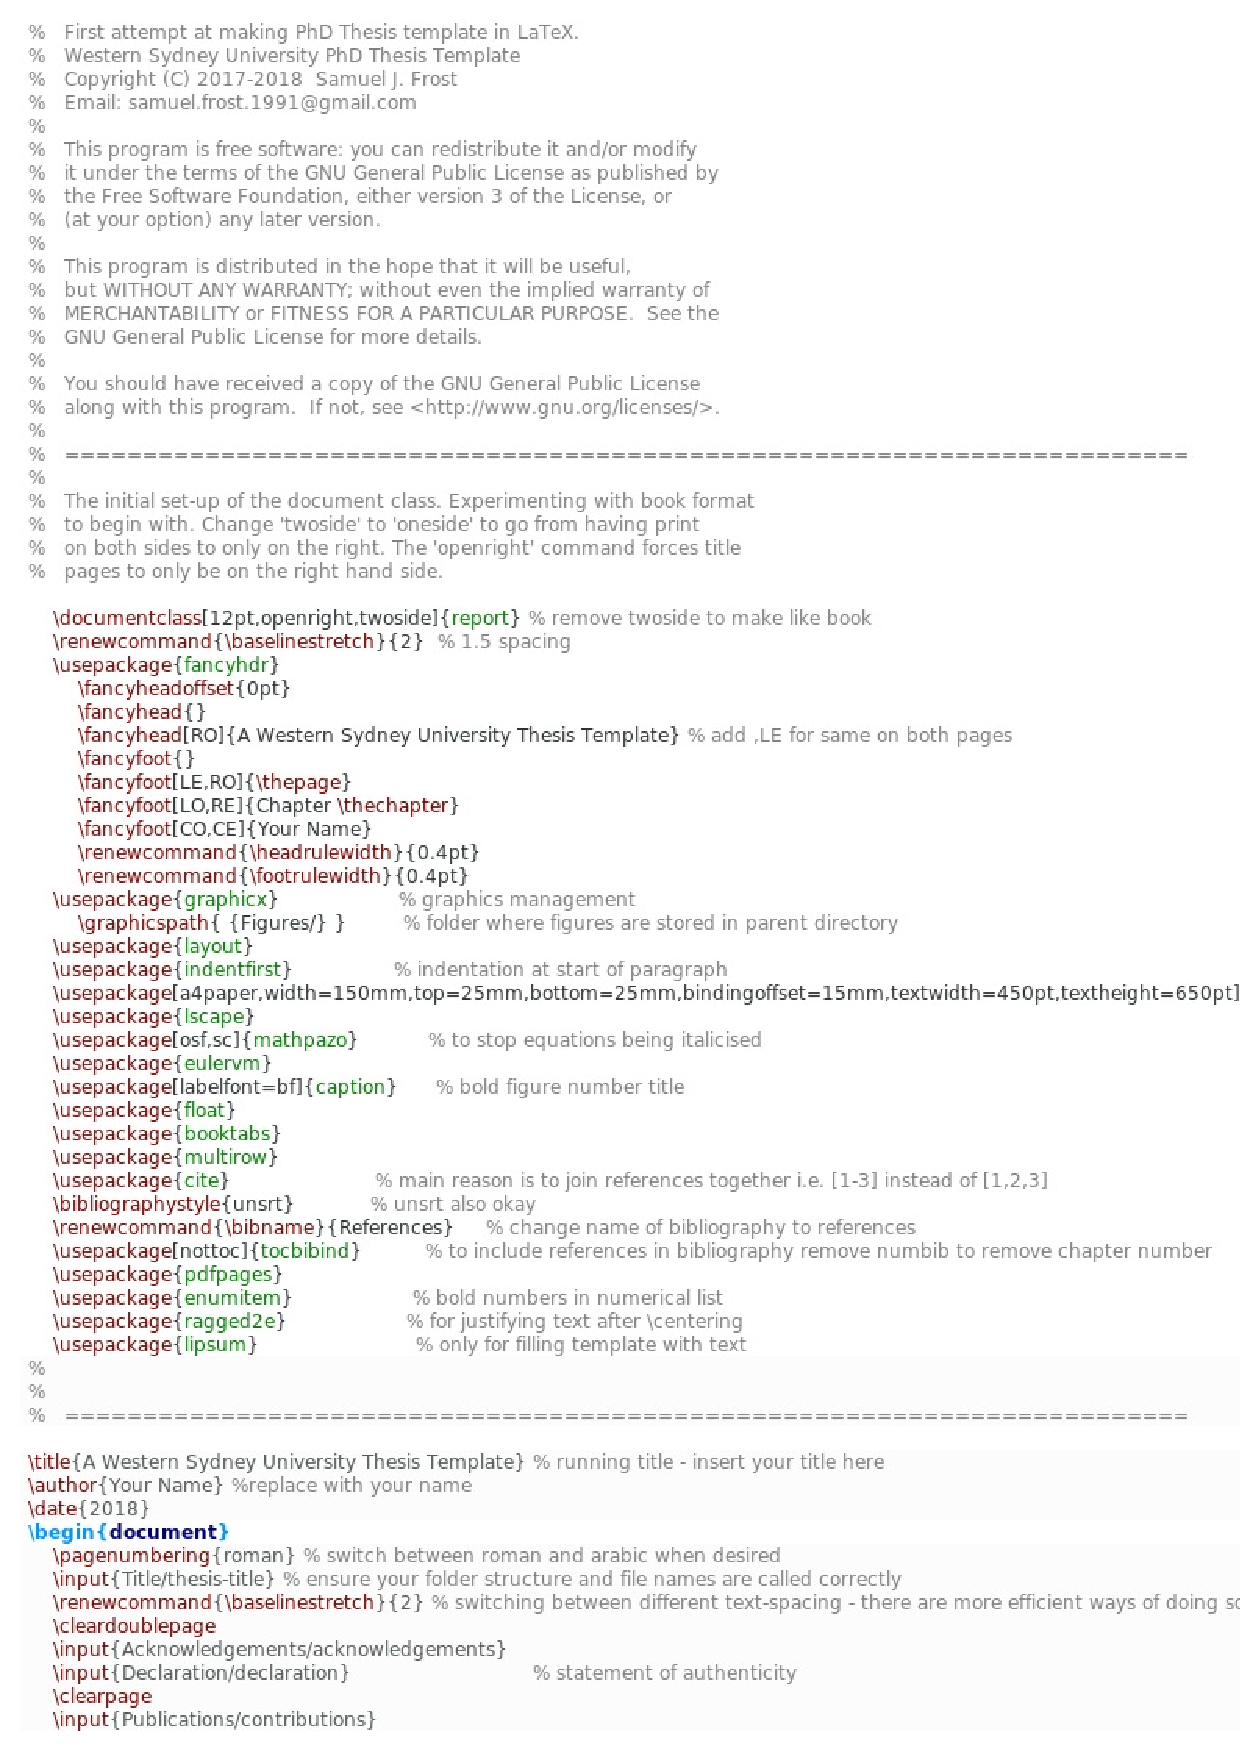
\includepdf[pages=-]{print.pdf} % this inputs the pdf into the final pdf, change the name to your pdf
	

\end{document}
